\documentclass[5pt]{article}
\usepackage{tikz}
\usepackage{CJKutf8}
\usetikzlibrary{positioning}
\usetikzlibrary{calc}
\usetikzlibrary{trees}
\begin{document}
\begin{CJK*}{UTF8}{gkai}
  
\begin{tikzpicture}[line width=3pt]
    \draw (0,0)|-(2,2);
    \fill[orange] (3,0) rectangle (5,2);
  \end{tikzpicture}

  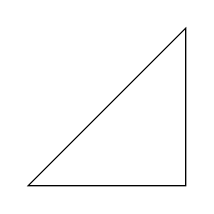
\begin{tikzpicture}
    \draw (0,0)--(2,2)--(2,0)--cycle;
  \end{tikzpicture}
  
  \begin{tikzpicture}
    \draw (0,0) rectangle (20pt,2);
  \end{tikzpicture}

  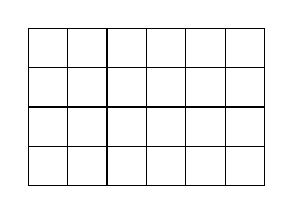
\begin{tikzpicture}
    \draw[step=0.5](0,0) grid (3,2);
  \end{tikzpicture}

  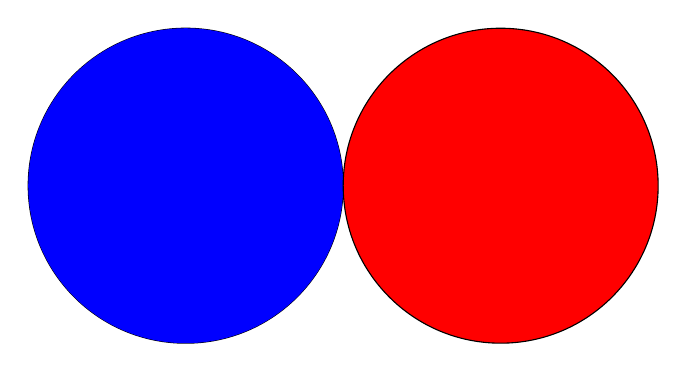
\begin{tikzpicture}
    \draw (0,0) circle (2);
    \fill[blue] (0,0) circle (2);
    \filldraw[fill=red] (4,0) ellipse (2 and 2);
  \end{tikzpicture}

  \begin{tikzpicture}
    \draw (0.5,0) arc (0:235:0.5);
    \draw (3,0) arc (0:270:2 and 2);
  \end{tikzpicture}

  \begin{tikzpicture}
    \draw (-2,2) parabola bend (0,0) (2,2);
  \end{tikzpicture}

  \begin{tikzpicture}
    \draw (0,0) sin (2,2) cos (2,0) sin (3,-2) cos (4,0);
  \end{tikzpicture}

  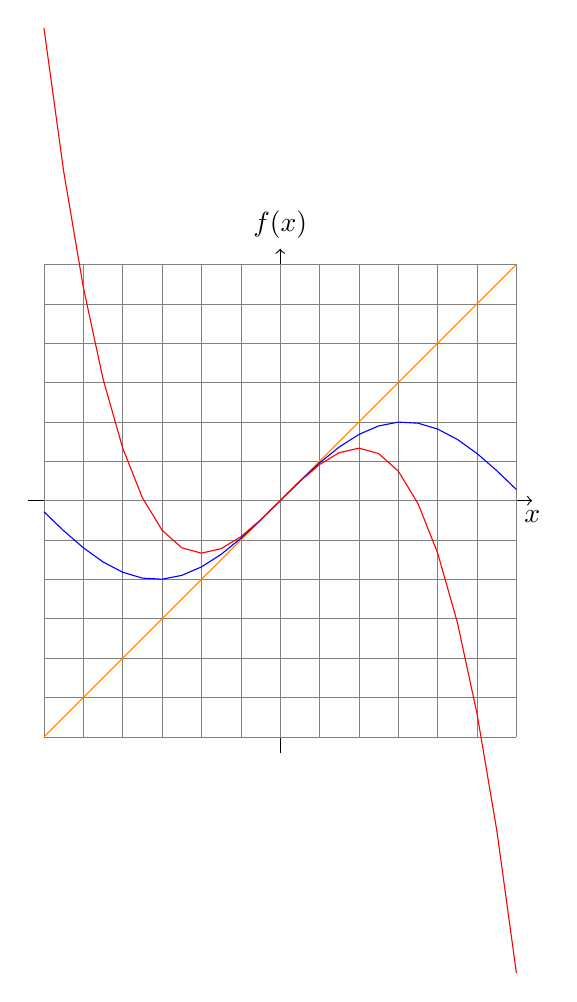
\begin{tikzpicture}[domain=-3:3]
    \draw[->] (-3.2,0)--(3.2,0) node[below] {$x$};
    \draw[->] (0,-3.2)--(0,3.2) node[above] {$f(x)$};
    \draw[very thin,color=gray,step=0.5](-3,-3) grid (3,3);
    \draw[color=orange] plot(\x,\x);
    \draw[color=blue] plot(\x,{sin(\x r)});
    \draw[color=red] plot(\x,{\x-(2/6)*(\x)^3});
  \end{tikzpicture}

  \begin{tikzpicture}[grow=right,
    level 1/.style={sibling distance=3cm},
    level 2/.style={sibling distance=1.5cm}]
    \node {A}[edge from parent fork right]
    child { node {B}
      child { node {G}}
      child { node {H}}
    }
    child { node {C}
      child { node {D}}
      child { node {E}}
    }
    child {node {F}};
  \end{tikzpicture}

  \begin{tikzpicture}[grow=right,
      level 1/.style={sibling distance=8cm},
      level 2/.style={sibling distance=4cm},
      level 3/.style={sibling distance=2cm},
      level 4/.style={sibling distance=1cm},
      level 5/.style={sibling distance=0.5cm}]
    \node[fill=lightgray]{玉超}[edge from parent fork right]
    child{node{大玉}}
    child{node{大亮}
      child{node{明进}}
      child{node{明号}
	child{node{应翠}
	  child{node{昌均}
	    child{node{炳盛}}
	    child{node{青松}}}
	  child{node{昌银}}
	  child{node{昌周}
	    child{node{培勇}}
	    child{node{培均}}
	    child{node{培林}}}
	  child{node{昌保}
	    child{node{体兵}}}}}
      child{node{明兴}
	child{node{应全}
	  child{node{昌松}
	    child{node{治荣}}
	    child{node{治富}}}
	  child{node{昌东}
	    child{node{治国}
	      child{node{朱威}}}}
	  child{node{昌培}
	    child{node{体富}
	      child{node{才见}}}}}}};
  \end{tikzpicture}
\end{CJK*}
\end{document}
